\chapter{Physical description of the climate system}
\section{Atmosphere}
The atmosphere is a gaseous envelope surrounding the Earth. It is composed of a mechanical mixture of several gases (like nitrogen and oxygen) and water vapor. Because is made of material particles, it exerts pressure due to the effects of gravity; because it is gaseous, the pressure decreases with height and the atmosphere is most dense near the ground

The atmosphere is characterized by a specific temperature profile. In the lower part, the general tendency of the temperature is to decrease with height. This region is called the troposphere, and it is the part directly connected with the Earth’s surface and is where most atmospheric processes usually associated with day-to-day weather take place. Above the troposphere, there is a region called the stratosphere, where the temperature, stays constant or increases with height. The division between the two regions is the tropopause, here the temperature often is its minimum for the vertical air column. In the region above, called the stratosphere, the temperature decreases with the height and after that in the thermosphere, the temperature continuously increases with the height. To understand how the atmosphere maintains this type of temperature vertical gradient, we have to take into consideration all the processes by which the atmosphere gains or loses energy and how these processes vary with latitude and season 

\subsection{Temperature profiles}
In the troposphere temperature decreases with $dT/dz=-6.4$ C/km on average.
\begin{table}[h]
\begin{tabular}{llll}
                                                             & {\color[HTML]{010066} \textbf{Troposphere (sum/win)}} & {\color[HTML]{010066} \textbf{Tropopause}} & {\color[HTML]{010066} \textbf{Stratosphere}} \\ \cline{2-4} 
\multicolumn{1}{l|}{{\color[HTML]{003532} \textbf{poles}}}   & 280 / 235                                             & 9 km: 230 / inversion (1.5/2 km)           & Slow Warming/ slow cooling                   \\
\multicolumn{1}{l|}{{\color[HTML]{003532} \textbf{midlat}}}  & 290 / 280                                             & 10 km: 220                                 & Slow Warming/ slow cooling                   \\
\multicolumn{1}{l|}{{\color[HTML]{003532} \textbf{tropics}}} & 300                                                   & 17 km: 190                                 & warming                                     
\end{tabular}
\end{table}

Inversion: because of strong surface cooling of air $\rightarrow$ inversion from the usual tropospheric and temperature decrease w/ height.

tropopause: temperature cte (where temp reaches the min for given air column)→190K at tropics
stratosphere: slight increase/ slight decrease



\section{Introduction}\label{introduction}

Sample citation of \citet{Richardson1922}.

The atmosphere is in motion and it is a continuous mixing and clashing
of vortices and structures, but when it is averaged over a long period
of time (fig.{\ref{fig:ERA5-wind200}}) it shows a remarkable simple structure.
The figure shows the wind at an approximate level of about 12km, that is
considered to be in the free atmosphere, far from the influence of the
ground. The circulation is a large vortex around the pole that shows
small oscillation in latitudes, especially pronounced over North America
and the Asian Pacific Coast. The flow is therefore predominantly in the
East-West direction, with a relatively small component in the meridional
direction. The \emph{circumpolar vortex} has been one of the first
structures to be recognized when plentiful observations of the upper air
flow became available, but it provided some of the intriguing questions
that drove the development of geophysical fluid dynamics to this time.
some of them have not been completely understood. What is maintaining
this peculiar circulation ? Which factor determines the amplitude and
location of the undulations in meridional direction ? Some of these
question will be addressed in these notes

\begin{figure}[h!]
    \centering
    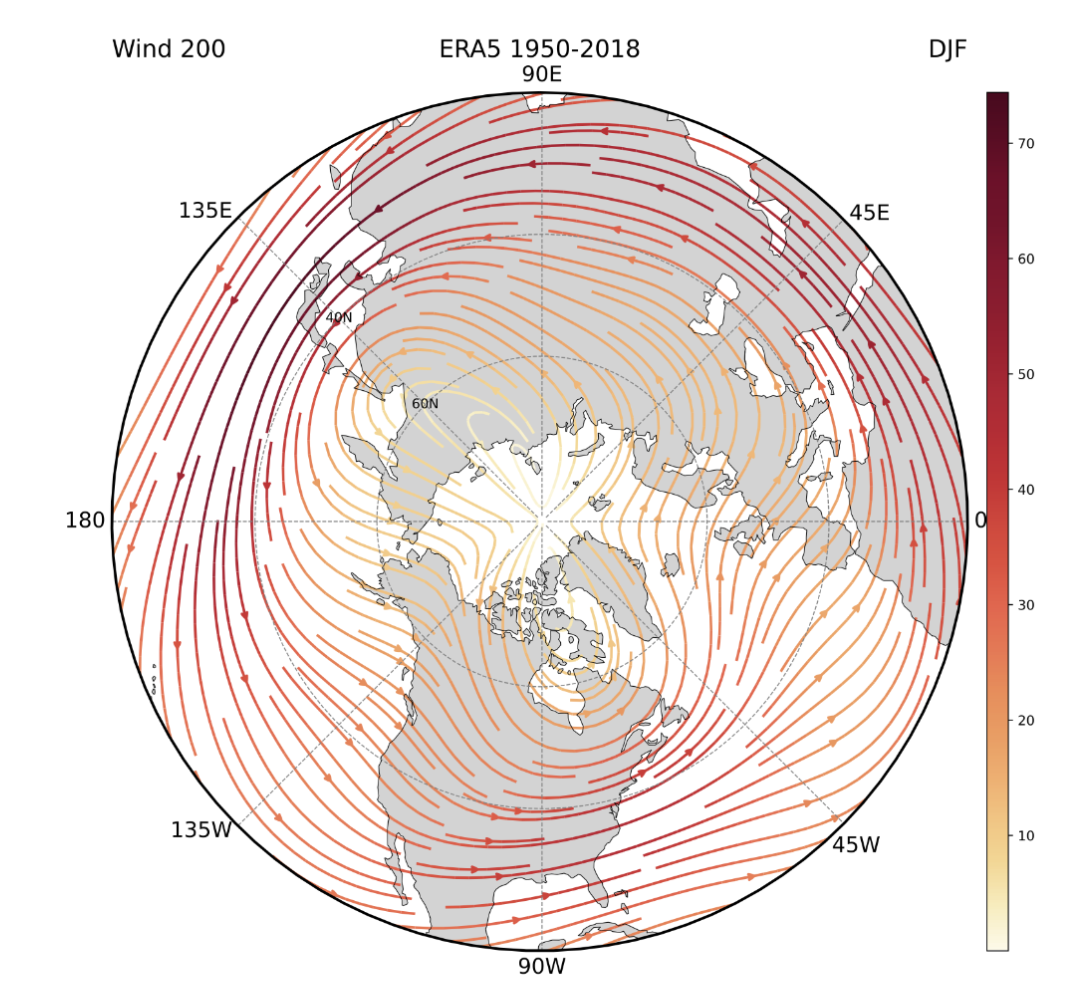
\includegraphics[width=0.5\linewidth]{uploads/Screenshot 2024-11-18 114256.png}
    \caption{ERA5-wind 200}
    \label{fig:ERA5-wind200}
\end{figure}


\subsection{Coordinate systems}\label{coordinate-systems}

\subsubsection{Spherical Coordinates}\label{spherical-coordinates}

The most commonly used coordinate system for the analysis of the
atmosphere and the oceans is a spherical coordinate system attached to
the rotating Earth (Fig. \texttt{fig:0} ). The spherical coordinates are
slightly different from the usual mathematical ones as the latitude is
measured from the equator and therefore it can take negative values. The
longitude is running west to east.

The longitude is also known as the ``zonal'' direction whereas the
latitude is also known as the "meridional" direction. Winds are
identified by the direction they are coming from, so a "westerly" wind
is coming \emph{from} the West and an "easterly" wind is coming from the
East.

This coordinate system is rotating with the Earth and therefore it
generates force terms in any dynamical equation expressed in this system
of coordinate, the Coriolis terms.

%\begin{figure}[h]
%    \centering
%    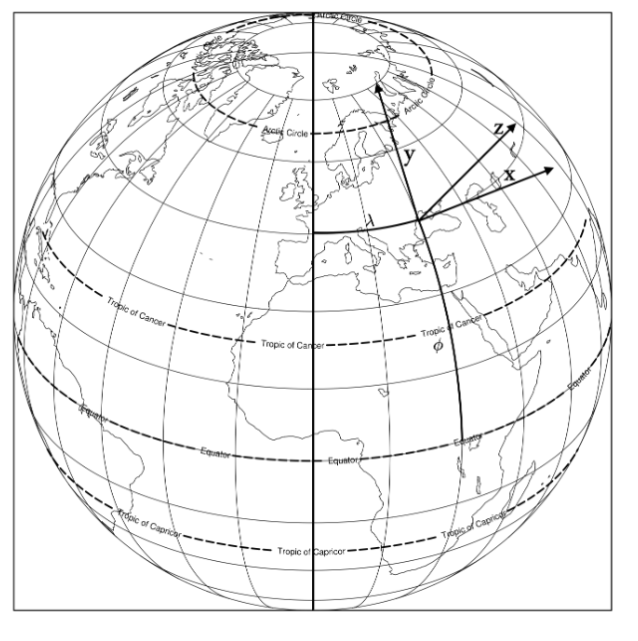
\includegraphics[width=0.5\linewidth]{uploads/Screenshot 2024-11-18 114156.png}
%    \caption{Coordinate system}
%    \label{fig:coordinate system3d}
%\end{figure}

\subsubsection{The Beta-plane}\label{the-beta-plane}

It is sometimes convenient to shift coordinate system if the latitudinal
extension of the motion is not too great with respect to the motion
parameters as they are expressed in the adimensional numbers. When this
is possible, a tangent coordinate system is applied at a specific
latitude \(\phi_0\) and the resultant Cartesian coordinates system is
called the \(\beta\)-plane. Usually symbols \((x,y)\) are used in this
case for the zonal and meridional coordinate. In the \(\beta\)-plane the
planetary vorticity \(f\) is linearized as \(f=f_0 + \beta y\), where
\(\beta = \frac{\partial f}{\partial y}({\phi_0})\).

\subsection{Advective derivative}\label{Sec:Adv}

To describe the governing equation of the atmosphere and eventually of
the ocean we have to understand how we write the rate of change with
time of this fluid. This problem was solved by considering the fact that
the rate of change in the fluid cannot be seen as arate of change with
respect to a fixed system of coordinate because the system is moving
with the fluid itself. Therefore, first we have to find a way to
describe the change taking into account the moving system of
restaurants. These can be done by using a concept developed in the 19th
century by Euler that is called "advective derivative" that can be
obtained from a total derivative of the property,

\[\frac{d \phi}{dt} = \frac{\partial \phi}{\partial t} + \frac{\partial x}{\partial t}\frac{\partial \phi}{\partial x} + \frac{\partial y}{\partial t}\frac{\partial \phi}{\partial y}+\frac{\partial z}{\partial t}\frac{\partial \phi}{\partial z} = \frac{\partial \phi}{\partial t} + \mathbf{v}\cdot\nabla\phi\]

and so it can be defined as

\[\frac{D \varphi}{Dt} =\frac{\partial \varphi}{\partial t} + \mathbf{v}\cdot\nabla\varphi\]

in this way the moving fluid can be described by derivatives with
respect the "fixed" coordinate system, i.e. the Eulerian description.
The alternative description of the observer moving with fluid is known
as the "Lagrangian" description.

\subsection{Primitive Equations}\label{Sec:Prim}

The equation governing the motion of the atmosphere can be written as:

\[\begin{aligned}
&\frac{D u}{Dt} -\frac{uv \tan{\phi}}{r} +  \frac{uw}{r} = -\frac{1}{\rho r \cos{\phi}}\frac{\partial p}{\partial \lambda} + fv - \hat{f}w + F_\lambda\\
&\frac{D v}{Dt} -\frac{u^2 \tan{\phi}}{r} +  \frac{vw}{r} = -\frac{1}{\rho r }\frac{\partial p}{\partial \phi} - fu  + F_\phi\\
&\frac{D w}{Dt} -\frac{u^2+v^2}{r} = -\frac{1}{\rho }\frac{\partial p}{\partial z} -g +\hat{f}u + F_z\\
\end{aligned}\]

the \(f=2\Omega \sin{\phi}\) and \(\hat{f} = 2\Omega\cos{\phi}\) terms
arise from the rotating spherical coordinate system that we have chosen,
other terms are generated by the spherical geometry. Some of them are
small and traditionally they can be neglected, so that we arrive at the
system

\[\begin{aligned}
&\frac{D u}{Dt} - v\left(f +  \frac{u \tan{\phi}}{a}\right)  = -\frac{1}{\rho a \cos{\phi}}\frac{\partial p}{\partial \lambda}   + F_\lambda\\
&\frac{D v}{Dt} + u\left( f + \frac{u \tan{\phi}}{a}\right)  = -\frac{1}{\rho a}\frac{\partial p}{\partial \phi}  + F_\phi\\
&\frac{D w}{Dt}  = -\frac{1}{\rho }\frac{\partial p}{\partial z} -g  + F_z\\
\end{aligned}\]

where we have also used the \emph{Shallowness Approximation} by assuming
\(r = a +z \approx a\), where \(a\) is the Earth radius.

However the advective derivative must be expressed in spherical
cordinates

\[\frac{D }{Dt} = \frac{\partial }{\partial t} + \frac{u}{a\cos{\phi}}\frac{\partial }{\partial \lambda} +\frac{v}{a}\frac{\partial }{\partial \phi} + w\frac{\partial }{\partial z}\]

so that the velocity components are

\[\begin{aligned}
&u = a\cos{\phi\frac{\partial \lambda}{\partial t}}\\
&v = a \frac{\partial \phi}{\partial t}\\
&w = \frac{\partial z}{\partial t}
\end{aligned}\]

These equation govern the mechanical behaviour of the atmosphere, and we
will see in a different form, also of the ocean. There three forces in
action: pressure gradient, rotaiton via the Coriolis force and gravity.

The equation are not complete,we have three equation but five variables,
so we need to find the missing relations. We are using the basic
conservation principles, the latter equations describe the conservation
of momentum, we can exploit the conservation of mass. The mass of the
fluid must be conserved locally, because there are now sinks or sources
in the atmosphere itself, so we want to write the mass of a volume of
atmosphere fixed in space as

\[M = \int_V  \rho \,dV\]

the mass in the volume can only change if there is a flux of mass at
surface \(S\),

\[\frac{\partial }{\partial t} \int_V  \rho \,dV = -\int_S \rho\mathbf{v}\cdot n \, dS\]

using the divergence theorem however we have

\[\frac{\partial }{\partial t} \int_V  \rho \,dV = -\int_V \nabla\cdot(\rho\mathbf{v}) \,dV\]

because the volume is not changing with time we can bring the derivative
inside the integral and we get

\[\int_V  \frac{\partial \rho}{\partial t}+\nabla\cdot(\rho\mathbf{v}) \,dV = 0\]

but the volume is arbitrary, so it must be that

\[\frac{\partial \rho}{\partial t}+\nabla\cdot(\rho\mathbf{v}) = 0\]

is valid locally.

We have still at our disposal the conservation of thermodynamical energy
and so we can also use

\[C_v\frac{D T}{Dt} = -p\frac{D }{Dt}\left(\frac{1}{\rho}\right)+ Q\]

where we included the temperature and heating/cooling term \(Q\). The
state variable are then linked by the state equation

\[p = \rho R T\]

where \(R\) is the gas constant for dry air.

We can use the equation of state to write the energy equation ( or the
temperature equation) in a different form,

\[c_v\frac{D T}{Dt} = -p\frac{D }{Dt}\left(\frac{R T}{p}\right)+ Q = -R\frac{D T}{Dt} + \frac{RT}{p}\frac{D p}{Dt} + Q\]

yielding the alternative forms ( since \(c_p = c_v +R\)),

\[c_p\frac{D T}{Dt}  - \frac{1}{\rho}\frac{D p}{Dt} = Q\]

For adiabatic processes \(Q=0\) and so

\[\begin{aligned}
&c_p\frac{D T}{Dt}  - \frac{1}{\rho}\frac{D p}{Dt} = 0\\
&\frac{c_p}{T}\frac{D T}{Dt} -\frac{R}{p}\frac{D p}{Dt} = 0\\
&\frac{D }{Dt}\log{T} - \frac{R}{c_p}\frac{D }{Dt}\log{p} = 0
\end{aligned}\]

integrating it we get

\[\log{T/T_0} - \log{\left(\frac{p}{p_0}\right)^{R/c_p}} = const\]

or

\[\frac{T}{T_0}\left(\frac{p_0}{p}\right)^{R/c_p} = const\]

so the quantity, known as \emph{potential temperature}

\[\theta = T\left(\frac{p_0}{p}\right)^{R/c_p}\]

is conserved in adiabatic processes and the thermodynamics equation can
be written as

\[\frac{D \theta}{Dt} = Q\]

\subsection{Hydrostatic balance}\label{hydrostatic-balance}

Under the action of gravity the vertical component of the pressure
gradient force balances the action of gravity, resulting in very small
vertical acceleration

\[\frac{\partial p}{\partial z} =  -g \rho\]

then if we take the vertical derivative of the eq. \texttt{Eq:logT}

\[\frac{1}{T_0}\frac{d T}{dz}\left(\frac{p_0}{p}\right)^{R/c_p} -\frac{p_0}{p^2}\frac{R}{c_p}\frac{T}{T_0}\left(\frac{p_0}{p}\right)^{R/c_p-1}\frac{d p}{dz} = 0\]

simplifying

\[\frac{d T}{dz} -\frac{p_0}{p^2}\frac{R}{c_p}T\left(\frac{p_0}{p}\right)^{-1}\frac{d p}{dz} = 0\]

or

\[\frac{d T}{dz} -\frac{1}{p}\frac{R}{c_p}T\frac{d p}{dz} = \frac{d T}{dz} +g\rho\frac{1}{p}\frac{R}{c_p}T = 0\]

but using the equation of state

\[\frac{d T}{dz} = -\frac{g}{c_p}\]

that gives how the temperature change with height under adiabatic
conditions and when the hydrostatic balance is valid. This is known as
the \emph{adiabatic lapse rate}.

\subsection{Summary of fundamental
equations}\label{summary-of-fundamental-equations}

Summarizing our discussion, the fundamental equation that describe the
motion of the atmosphere then are:

\[\begin{aligned}
&\frac{D u}{Dt} - v\left(f +  \frac{u \tan{\phi}}{a}\right)  = -\frac{1}{ a \cos{\phi}}\frac{1}{\rho}\frac{\partial p}{\partial \lambda}   + F_\lambda \\
&\frac{D v}{Dt} + u\left( f + \frac{u \tan{\phi}}{a}\right)  = -\frac{1}{a}\frac{1}{\rho}\frac{\partial p}{\partial \phi}  + F_\phi \\
&\frac{D w}{Dt}  = -\frac{1}{\rho }\frac{\partial p}{\partial z} -g  + F_z \label{Eq:PrimEq}\\
&\frac{D \theta}{Dt} = Q \\
&\frac{\partial \rho}{\partial t}+\frac{1}{a\cos{\phi}}\left[ \frac{\partial }{\partial \lambda}(\rho u) + \frac{\partial }{\partial \phi}(rv\cos{\phi} \right] +\frac{\partial }{\partial z}(\rho w) = 0 \\
&p = \rho R T
\end{aligned}\]

where we have used the divergence in spherical coordinates.

These equations are still not closed because we will need to express the
heating/cooling term \(Q\) and the friction terms \(F\) as a function of
the state variables. This will require a theory of the processes that
drive them. Where \(R=287.052874 J \quad kg^{-1} K^{-1}\) is the gas
constant for dry air and \(c_p = 1.005\) is the specific heat at
constant pressure, \(c_v = 0.718\) is the specific heat at constant
volume, \(\kappa = \frac{R}{c_p}\) and \(\gamma=c_p/c_v\) is their
ratio.

For theoretical and idealized studies the set of equation projected on
the \(\beta\)-plane is also used

\[\begin{aligned}
&\frac{D u}{Dt} - fv  = -\frac{1}{\rho}\frac{\partial p}{\partial x}   + F_x \\
&\frac{D v}{Dt} + fu = -\frac{1}{\rho}\frac{\partial p}{\partial y}  + F_y \\
&\frac{D w}{Dt}  = -\frac{1}{\rho }\frac{\partial p}{\partial z} -g  + F_z \\
&\frac{D \theta}{Dt} = Q\\
&\frac{\partial \rho}{\partial t}+\nabla\cdot(\rho\mathbf{v}) = 0\\
&p = \rho R T
\end{aligned}\]

and the gradient operator is the cartesian operator

\[\nabla = \frac{\partial }{\partial x} + \frac{\partial }{\partial y} + \frac{\partial }{\partial z}\]

and the advective derivative is then

\[\frac{D }{Dt} = \frac{\partial }{\partial t} + u\frac{\partial }{\partial x} + v\frac{\partial }{\partial y} + w\frac{\partial }{\partial z}\]


\section{The General Circulation of the
Atmosphere}\label{chp:GeneralCirculation}

Since heated air tends to rise and low-level ait must flow in to replace the risen heated air, the relative heating and cooling of different areas in the Earth’s surface, plays a significant role in driving local winds and the large-scale atmospheric circulation. The atmospheric circulation can be sum up into two different contributes: the east-west motion of the Walker circulation and the north-south circulation of the Hadley, Ferrel and polar cells. 

- The Walker circulation refers to the equatorial Pacific and involves rising air over the region of Indonesia and descending air over the eastern Pacific. It was examined following the discovery of strong negative correlation between surface pressure anomalies in the two regions. 

- The tropical Hadley cell is driven by solar heating, causing rising motion near the equator, then by the release of latent heat as the rising air leads to precipitation in the rising-air branch of the cell. This rising-air branch of the Hadley cell is not centered consistently on the equator but migrates north and south with the seasons. Moreover, the strength of the Hadley circulation varies with longitude, being strongly affected by such factors as whether the underlying surface is land or ocean. After rising near the equator, the air in the Hadley cell moves poleward, sinking near 30°N and 30°S and thereby generating belts of surface-level high pressure near 30°N and 30°S. Since the sea level pressure is low, the high pressure produced by the sinking air at about 30°N and 30°S creates a surface pressure gradient leading to the movement of a portion of the sinking air back toward the low pressure near the equator. The region of low-level convergence toward the bottom of the rising-air branch of the Hadley cell is called the intertropical convergence zone (ITCZ). 

- In the mid-latitude Ferrel cell, termed indirect because of having rising air in its cooler branch, the low-level flow is toward the poles, away from the relatively high pressure produced by the descending arms of the Hadley and Ferrel cells at about 30° latitude and toward the relatively low pressure at about 60° latitude. 

- The third cell in the three-cell pattern is the polar cell. Strong radiational cooling near the poles, causes polar air to become cold and dense, which in turn causes it to sink. Thus there is relatively high pressure at the pole, which, combined with the low pressure near 60°N and 60°S discussed in connection with the rising-air branch of the Ferrel cell, produces surface flow equatorward from the pole. This polar cell is extremely weak, although it remains detectable in time averages of the air circulation. 

What is more, you have to take into consideration the Coriolis effect, for which the rotation of the Earth causes moving air to be deflected to the right in the Northern Hemisphere and to the left in the Southern Hemisphere. 

\subsection{Space-time splittings}\label{space-time-splittings}

The dominant shape of the global circulation suggest that some
understanding can be gained from splitting the physical fields in larger
and smaller portions using appropriate averages. At a first inspection
the flow is seen as a predominant circumpolar vortex with superposed
fluctuations in space and time. The longitudinal directions i also known as the "zonal" direction, therefore the average over longitude is known
as the zonal averaging.

\subsection{Zonal means}\label{zonal-means}

The zonal mean of a quantity \(A\) is defined as the average over
longitudes. Commonly used symbols int he literature are the overbar
(\(\bar{u}\)) or square brackets ((\([u]\)), the first is most
frequently encountered in the theoretical and modeling literature
whereas the second is most commonly used in observational and
diagnostics works. In the following we will use brackets.

\[[A] = \frac{1}{2\pi}\int_0^{2\pi} A \, dx\]

so that the total field can be decomposed as

\[A = [A] + A^*\]

where \(A^*\) is the deviation from the zonal mean. The average has the
properties that \([[A]] = [A]\) and \([A^*]=0\).

When a streamfunction can be defined, the average zonal mean meridional
velocity is zero:

\[= \frac{1}{2\pi}\int_0^{2\pi} v \, dx=\frac{1}{2\pi}\int_0^{2\pi} \frac{\partial \psi}{\partial x} \, dx=0\]

This is a consequence of the more general result that the zonal mean of
any quantity that is a longitude derivative is zero.

\subsection{Time means}\label{time-means}

The time mean is defined simply as the average over a length of time.
Also in this case several common symbols are used, once again the
overbar or sometimes curly brackets, in the following we will use the
overbar

\[\bar{A} = \frac{1}{T}\int_0^{T} A \, dt\]

so that the total field is

\[A = \bar{A} + A'\]

The deviations from the zonal means are called "eddy" components. An
eddy that obeys a dispersion relation is a "wave".

\subsection{Higher order quantities}\label{Sect:Higher}

The averages can be used to decompose higher order quantities. For
instance using zonal means a quadratic correlation of the form \(A B\)
can be decomposed as

\[A B = ([A]+A^*)([B]+B^*) = A^*B^* + [A] B^*+ A^*[B] + [A][B]\]

taking a further zonal mean we get

{\[= [A^*B^*+ [A]B^* + A^*[B] + [A][B]] =  [A][B] + [A^*B^*]\]}

because the mix terms disappear as the average of the deviations is
zero.

We can refine the splitting by considering the time average splitting of
the zonal terms:

\[\begin{aligned}
= \bar{[A]} + [A]' \\
A^* = \bar{A}^* + A'^*
\end{aligned}\]

These terms represent the stationary symmetric circulation, the
transient symmetric circulation and the stationaty deviation from the
zonal means ("asymmetries") and the transient asymmetries.

Inserting these relations into Eq.(\texttt{AB1}) we get

\[= (\bar{[A]} + [A]')(\bar{[B]} + [B]') + [A^*B^*]\]

the time mean of the terms linear in the time deviation will average
again to zero (this time with respect the time mean) and we finally get

\[\overline{[AB]} = \bar{[A]}\bar{[B]} + \overline{[A]'[B]'} + \overline{[A^*B^*]}\]

The decompositions are not unique. We have first performed the split in
the zonal mean and then the split in the time mean, considering a split
only in the eddy part:

\[A^* =    \bar{A}^* + A'^*\]

we would get

\[[ \overline{AB}] = \bar{[A]}\bar{[B]} +  [\bar{A}^*\bar{B}^*]+[\overline{A'^*B'^*} ]\]

where the first term is the contribution of the mean meridional
circulation, thr second is the contribution of the time-mean
(\emph{standing}) eddies and the last one is the contribution of the
transient eddies.

This kind of decomposition is therefore a useful instrument, but
requires always consideraiton of the hypothesis formulated in the
initial design. Another consideration is that they depend on the
psecific kind of averaging that is used. There is little choice in the
zonal mean, being fixed by the geometry, but we have much more choices
in the case of the time mean. Results will depend on the length of the
time averaging period and on the original frequency of the data.Time
mean and second order quantities calculated over daily will differ from
the same quantities calculated over time series of weekly or monthly
data.

There is no \emph{correct} choice, each one will offer a different
glimpse in the data from a chosen perspective.

\subsection{The time averaged zonal general
circulation}\label{the-time-averaged-zonal-general-circulation}

The picture of the time averaged circulation is shown in Fig.
(\texttt{fig:51}). The picture has been computed from the data of the
ERA5 Reanalysis {[}add reference{]}. It i spossible to see the westerly
mid-atmosphere jets, located in the subtropical region at approximately
\(30\circ\) north and south. They show a maximum well in the interior of
the fluid around the 200mb level ( about 12 km). The westerly floe
extend to the ground in the mid-latitudes, whereas the equatorial zone
is occupied by easterly flows.

The jets have a strong seasonal cycle that result in an accelerated jet
in Winter in both hemispheres and relatively weaker jets in the Summer.
The jets show a seasonal poleward migration of the core of the flow,
with a generally more concentrated and intense maximum in the winter
season. The Southern hemisphere winter jet is wider then its counterpart
in the Northern Hemisphere, but they are both clearly linked to the
stratospheric flow above. The stratosphere also shows strong jets with
an even stronger seasonal cycle, with easterlies substituting the
westerlies from one season to the the next.

\begin{figure}[h!]
    \centering
    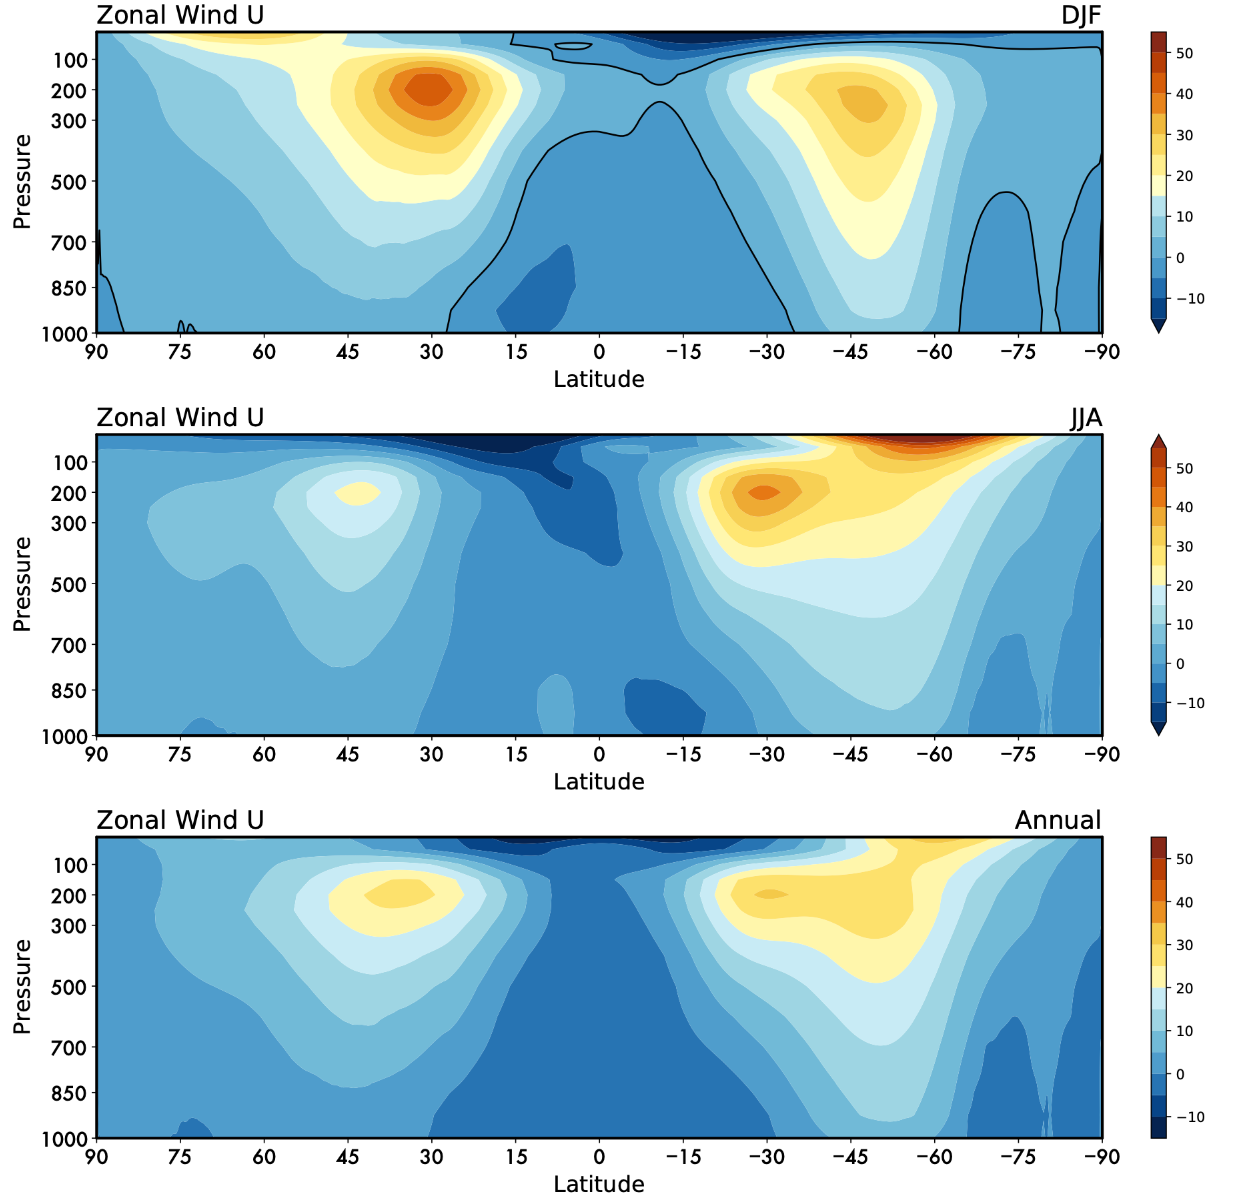
\includegraphics[width=0.5\linewidth]{uploads/Screenshot 2024-11-18 124309.png}
    \caption{Uzonal}
    \label{fig:Uzonal}
\end{figure}

The zonally averaged meridional circulation is shown in
Fig.(\texttt{fig:52}). It is possible to see the low level convergence
at the equator and high level divergence of the flow. The annual mean
show more clearly the direct circulation that is located between the
tropics. Note that the point of convergence, the InterTropical
Convergence Zone  ITCZ, though is generally following the seasonal
cycle of the sun is asymmetric with respect the equator, oscillating
between \(15N\) and \(5S\).

\begin{figure}[h!]
    \centering
    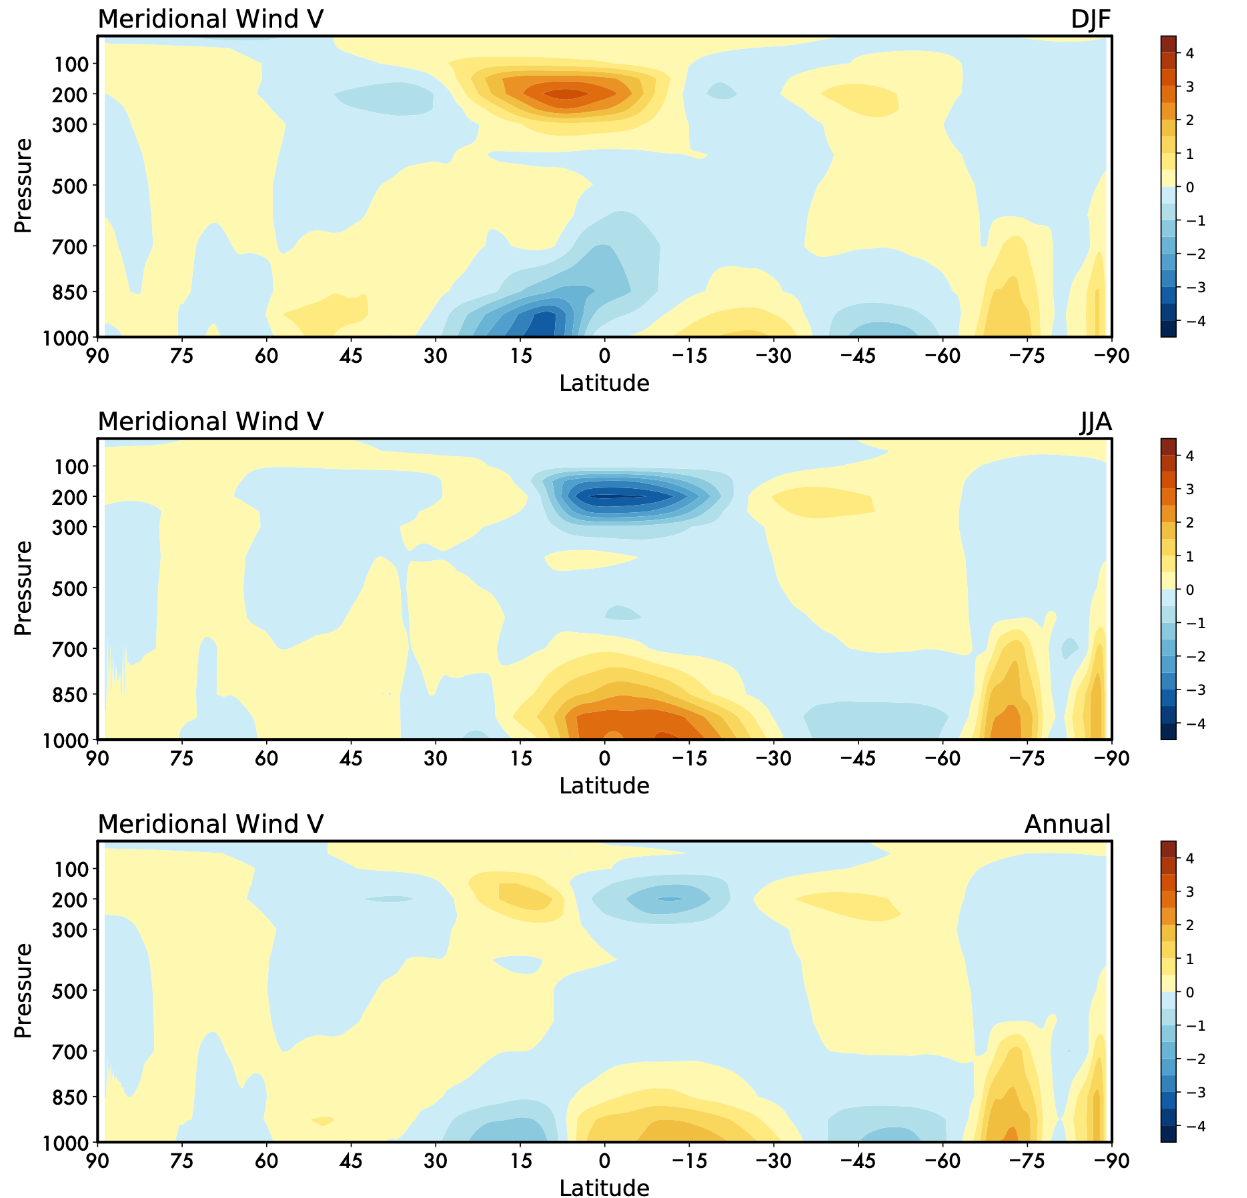
\includegraphics[width=0.5\linewidth]{uploads/Screenshot 2024-11-18 124445.png}
    \caption{Vzonal}
    \label{fig:Vzonal}
\end{figure}


The thermal structure is shown in Fig. \texttt{fig:53}. As a consequence
of the radiation balance the temperature is decreasing with latitude.
The equatorial area is receiving excess radiation with respect to the
the polar region. The hydrostatic balance is shown in the decreasing
temperature with height, but the lapse rate is less than adiabatic,
indicating the average stable nature of the atmosphere. There is a
strong latitudinal gradient in temperature, but the gradient is
decreasing with altitude and is actually reversing sign in the upper
atmosphere and stratosphere.

This is caused by the radiation absorption by ozone and other components
in the lower stratosphere. The change of sign of the temperature
meridional gradient Fig. \texttt{fig:531} is also consistent with the
structure of the zonal wind, with positive shear in the troposphere and
negative shear above it, consistent with the thermal wind balance.

\begin{figure}[h!]
    \centering
    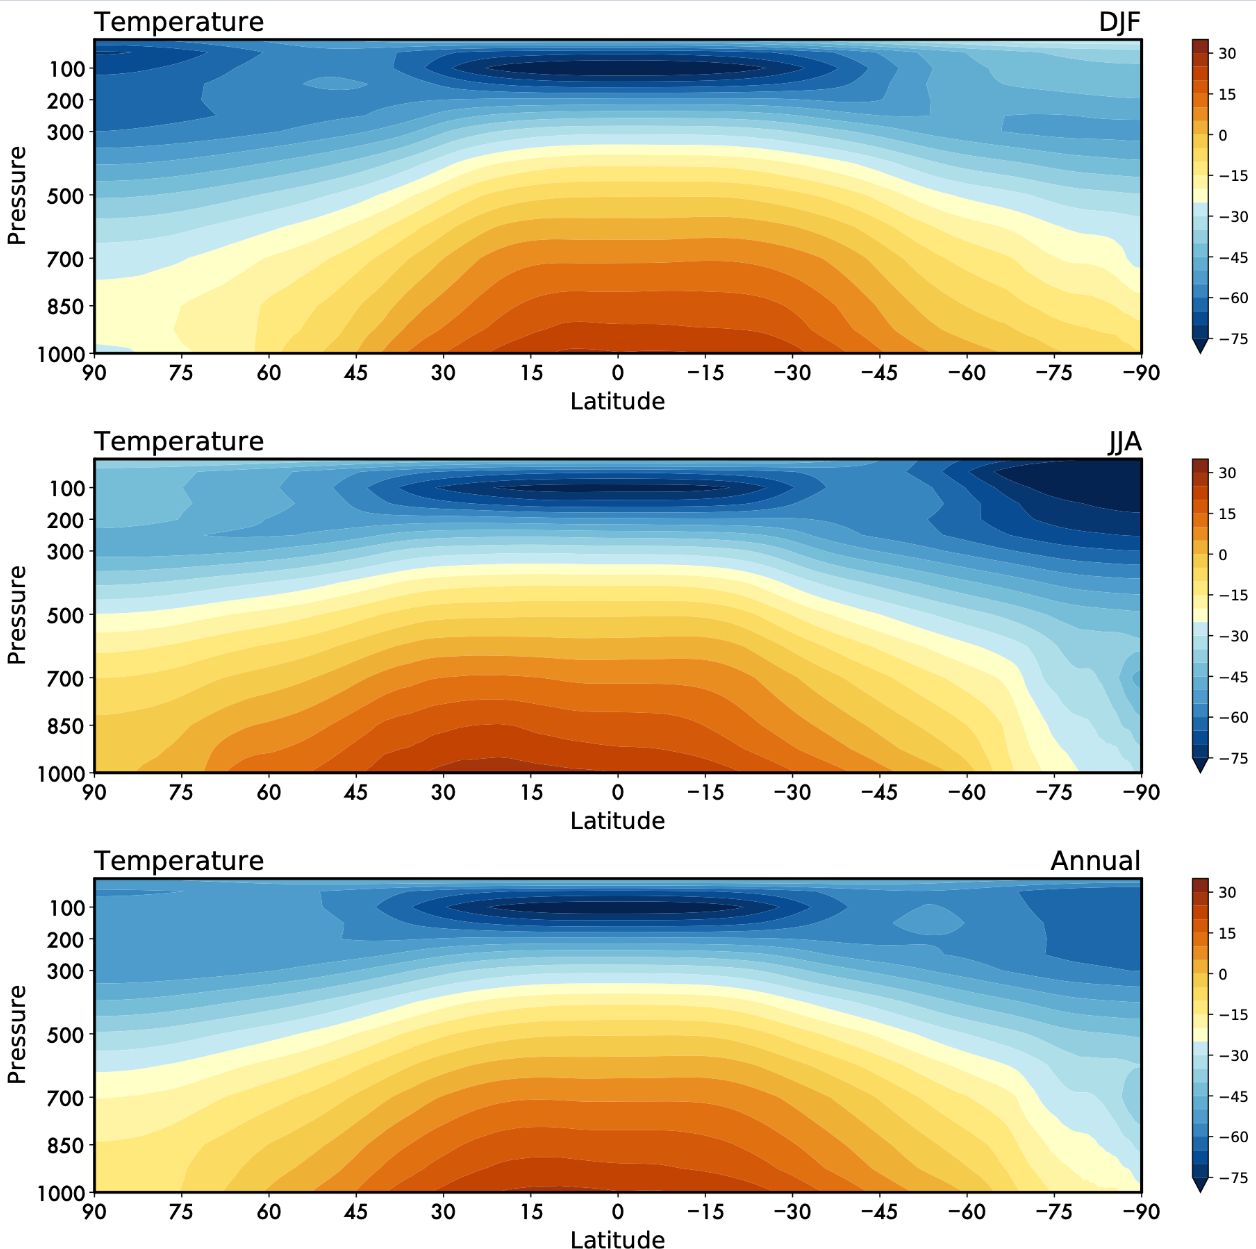
\includegraphics[width=0.5\linewidth]{uploads/Screenshot 2024-11-19 131634.png}
    \caption{Tzonal}
    \label{fig:enter-label}
\end{figure}
\begin{figure}[h!]
    \centering
    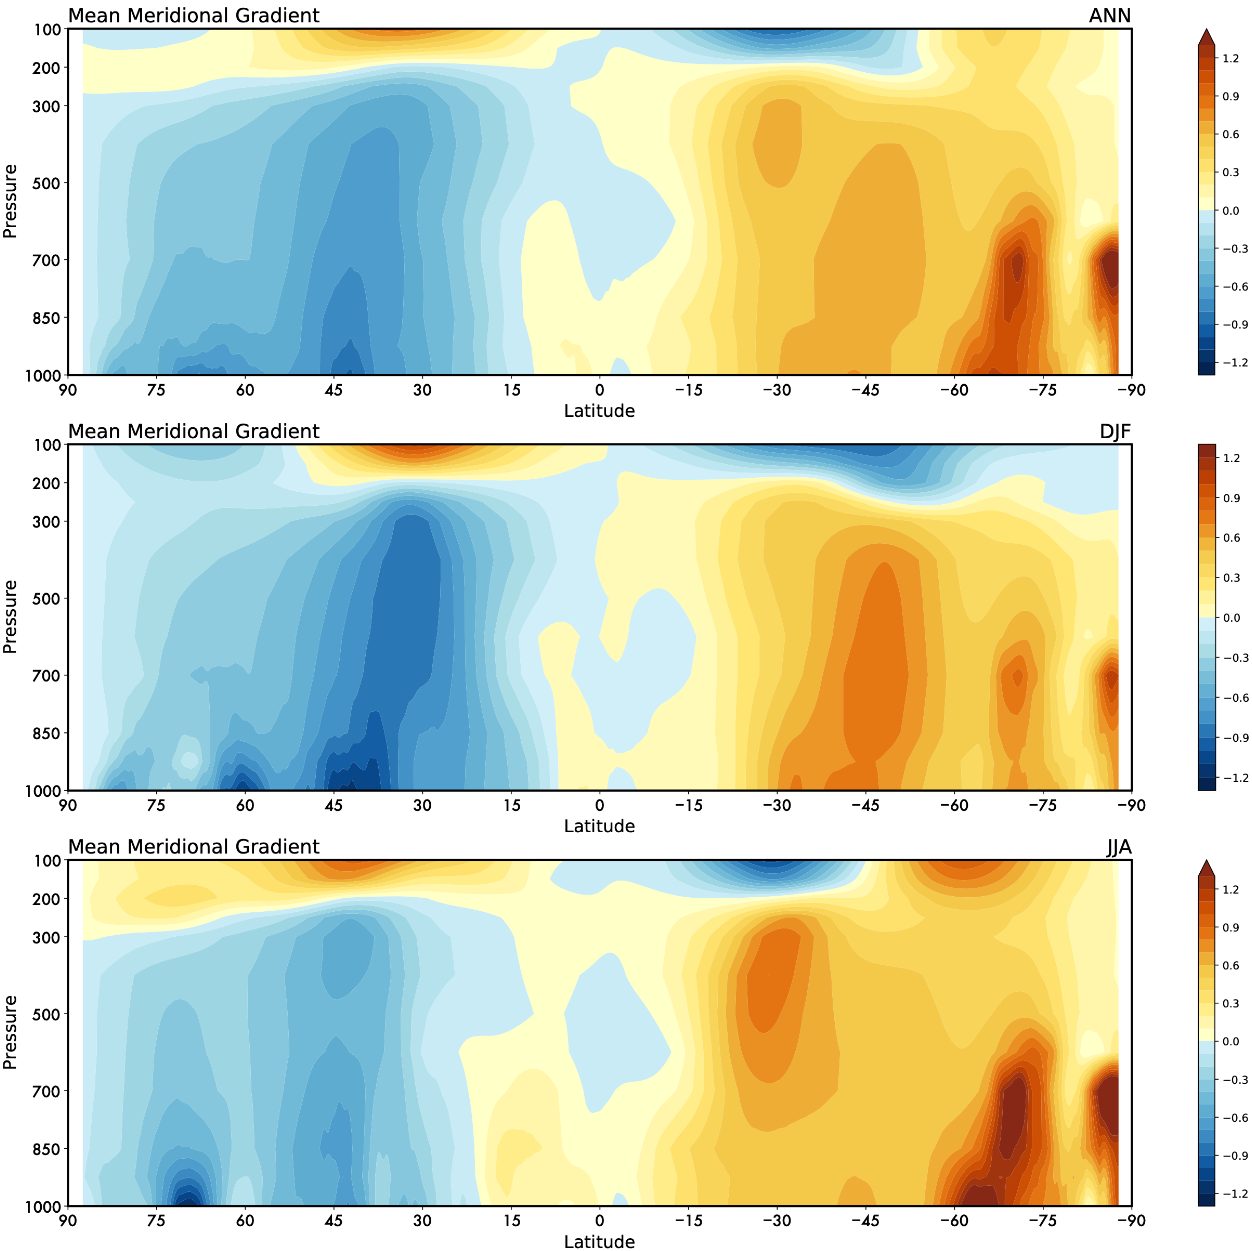
\includegraphics[width=0.5\linewidth]{uploads/Screenshot 2024-11-19 131845.png}
    \caption{Tgradient}
    \label{fig:enter-label}
\end{figure}


The structure of the distribution of water vapor in the atmosphere is
shown in Fig. \texttt{fig:532}. The water vapor is shown as the
\emph{specific humidity} that is mass of water vapour in a unit mass of
moist air, usually expressed as grams of vapour per kilogram of air. The
annual average (bottom) shows how the water vapor is strongly confined
to the lower levels and to the equatorial zone. The atmosphere is very
dry as the altitude increases. This is a direct consequence of the
strong dependence on temperature of the Clausius-Clayperon equation that
describes how the saturation water vapor pressure changes with
temperature. At the equator, really moist air contains 12-15 grams of
water per kilogram of moist air.

The seasonal distributions (other panels in Fig. \texttt{fig:532}) show
a shift of specific humidity in latitude roughly following the seasonal
cycle of the sun. The surface maximum is located around 5S in DJF and
then shifts to around 10N in JJA. The Winter hemisphere in both seasons
is definitely more moist at the surface than the Summer, but values are
smaller than the equatorial zone, reaching at most around 8 g/kg.

\begin{figure}[h!]
    \centering
    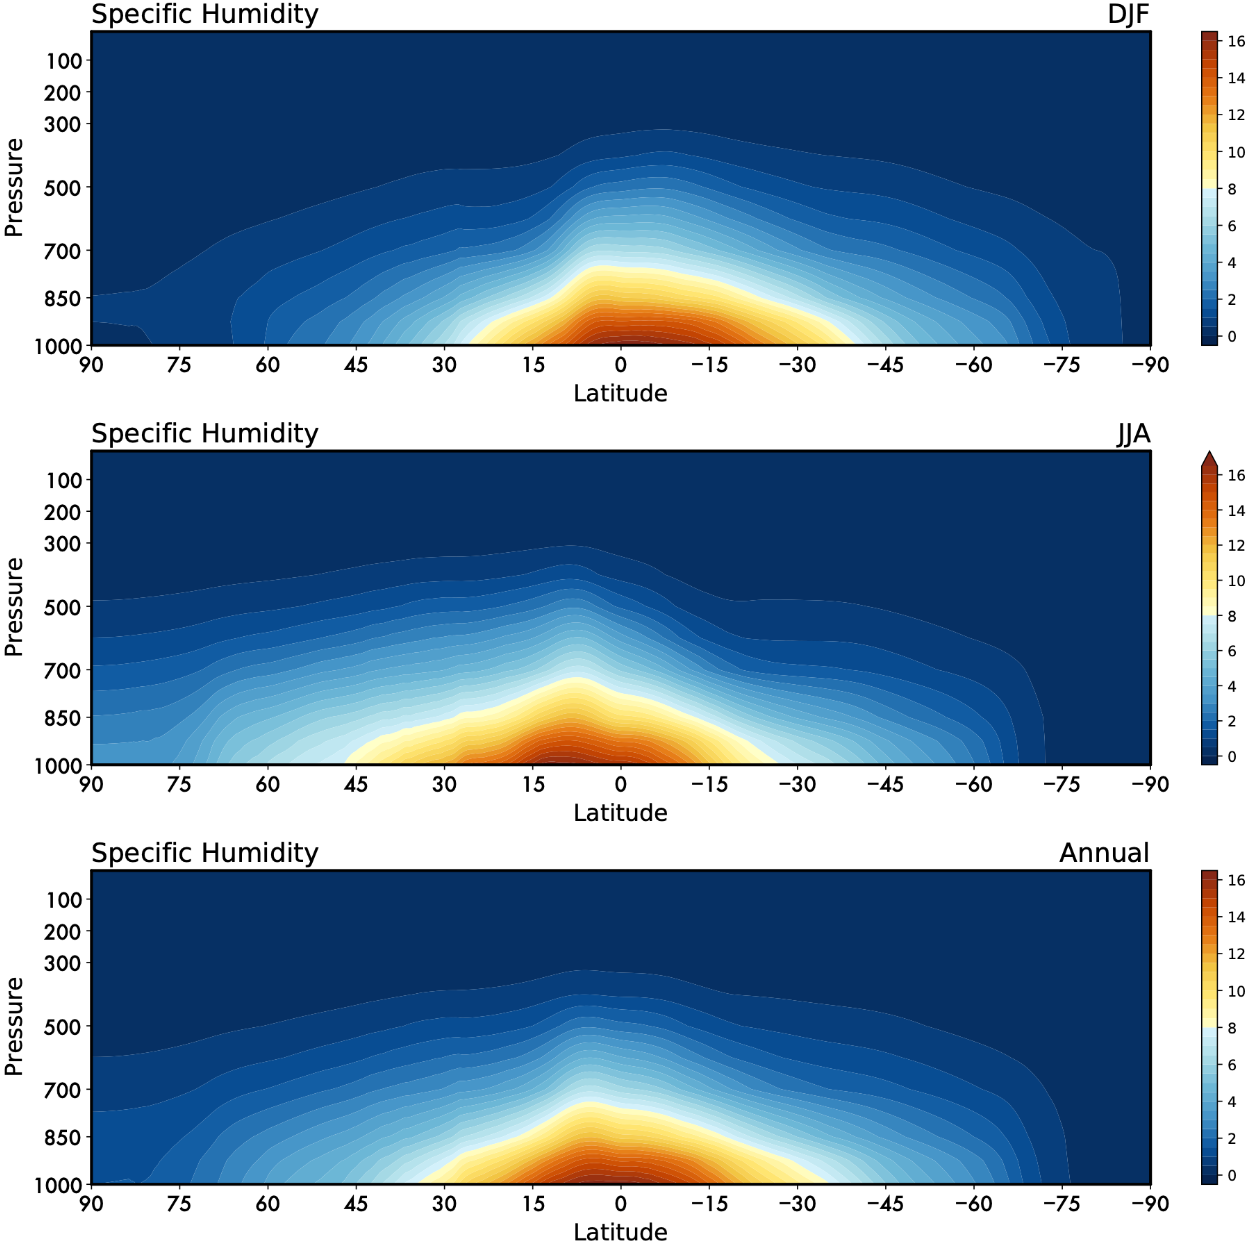
\includegraphics[width=0.5\linewidth]{uploads/Screenshot 2024-11-19 132133.png}
    \caption{Qzonal}
    \label{fig:enter-label}
\end{figure}

. {[}fig:532{]}

\begin{figure}[h!]
    \centering
    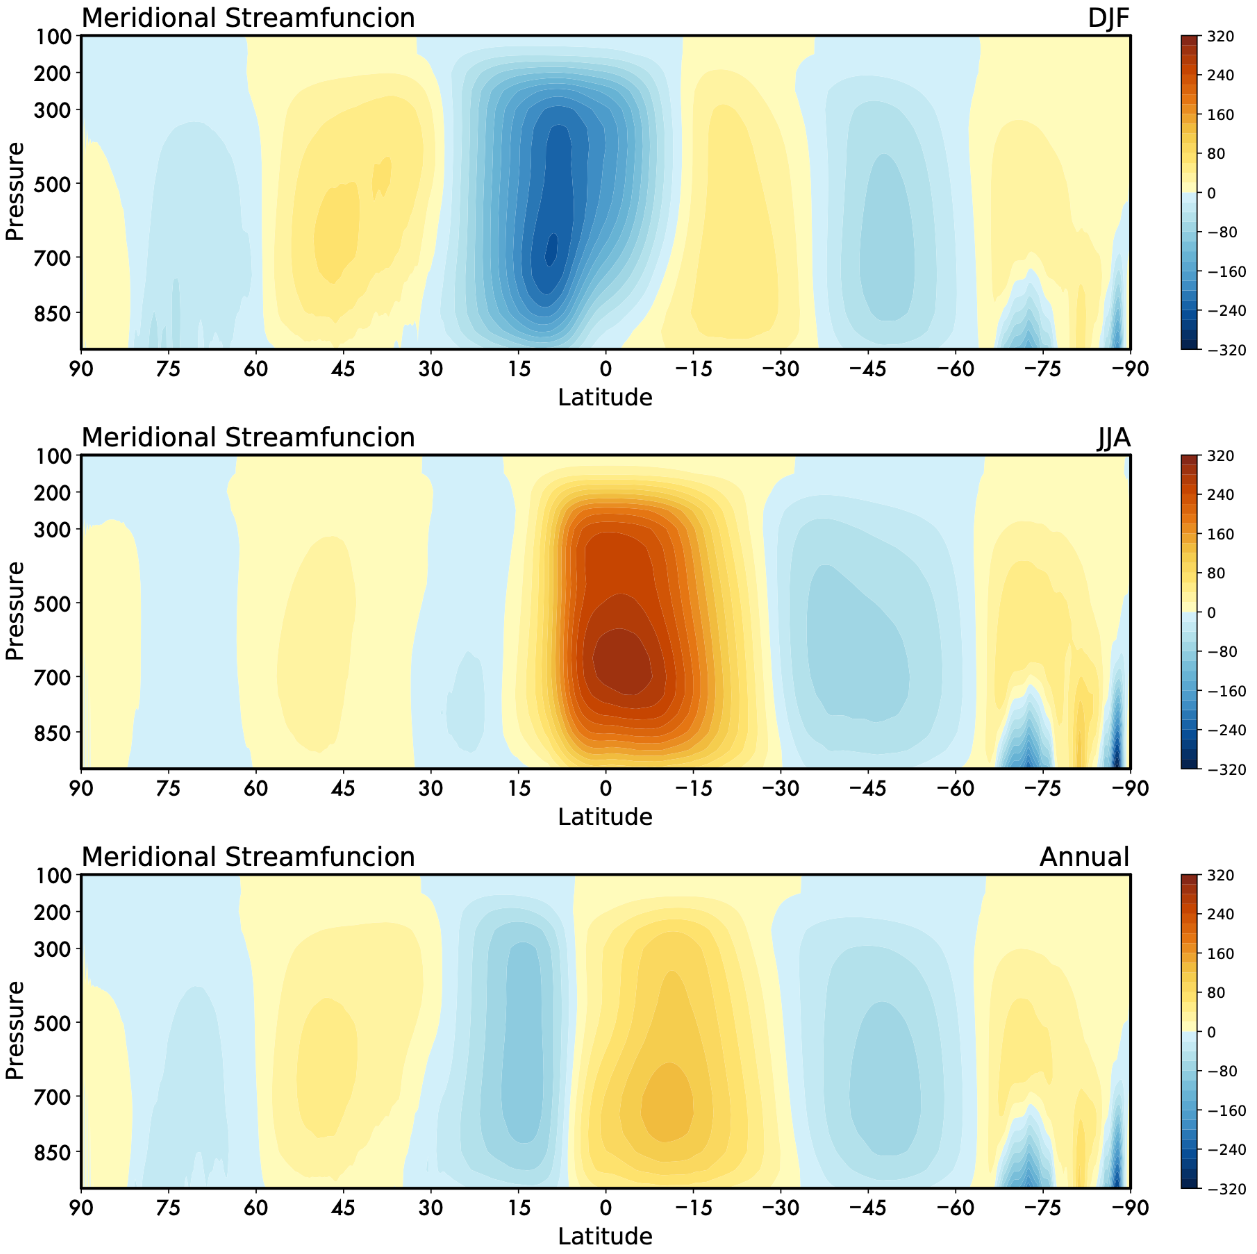
\includegraphics[width=0.5\linewidth]{uploads/Screenshot 2024-11-19 132224.png}
    \caption{MSzonal}
    \label{fig:enter-label}
\end{figure}


\subsection{The horizontal general
circulation}\label{the-horizontal-general-circulation}

Fig. \texttt{fig:551} shows the climatological geopotential height for
DJF at 200mb. The top panel shows the full field. The geostrophic
balance implies that it can be considered as an approximate
streamfunction for the horizontal flow. The bottom panel shows the same
field with the zonal mean removed, the eddy component. It shows clearly
the large deviations from the zonally symmetric circulation located over
the east coast of continents. A more careful inspection may reveal that
they are downstream from large continental size mountain ranges, the
Rocky Mountains and the Himalayan Plateau.

\begin{figure}[h!]
    \centering
    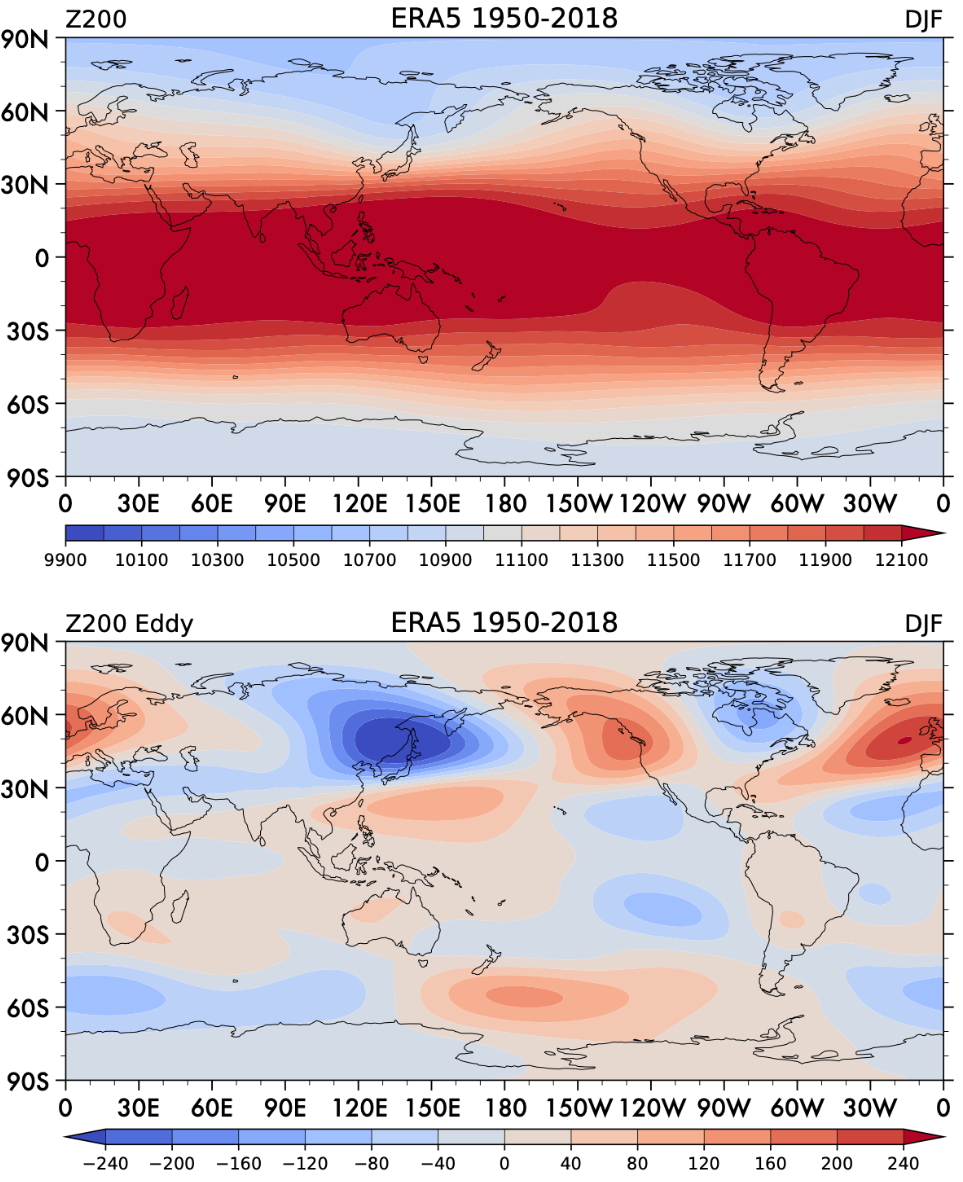
\includegraphics[width=0.5\linewidth]{uploads/Screenshot 2024-11-19 132329.png}
    \caption{Z200}
    \label{fig:enter-label}
\end{figure}

A better insight is provided by using a special polar projection to
inspect the Geopotential field. There are several geographical
projection to represent quantity on the sphere on a map and each of them
is useful to enhance some property of the flow. The shape of the
hemispheric circumpolar vortex is for instance clearly represented in
the stereo projection of Fig. \texttt{fig:552}. it is possbile to see
the curvature of the flow downstream of the Rocky Mountains and the
Himalayas and the typical shape of the Winter climatological pattern of
the high altitude atmospheric geopotential.

\begin{figure}[h!]
    \centering
    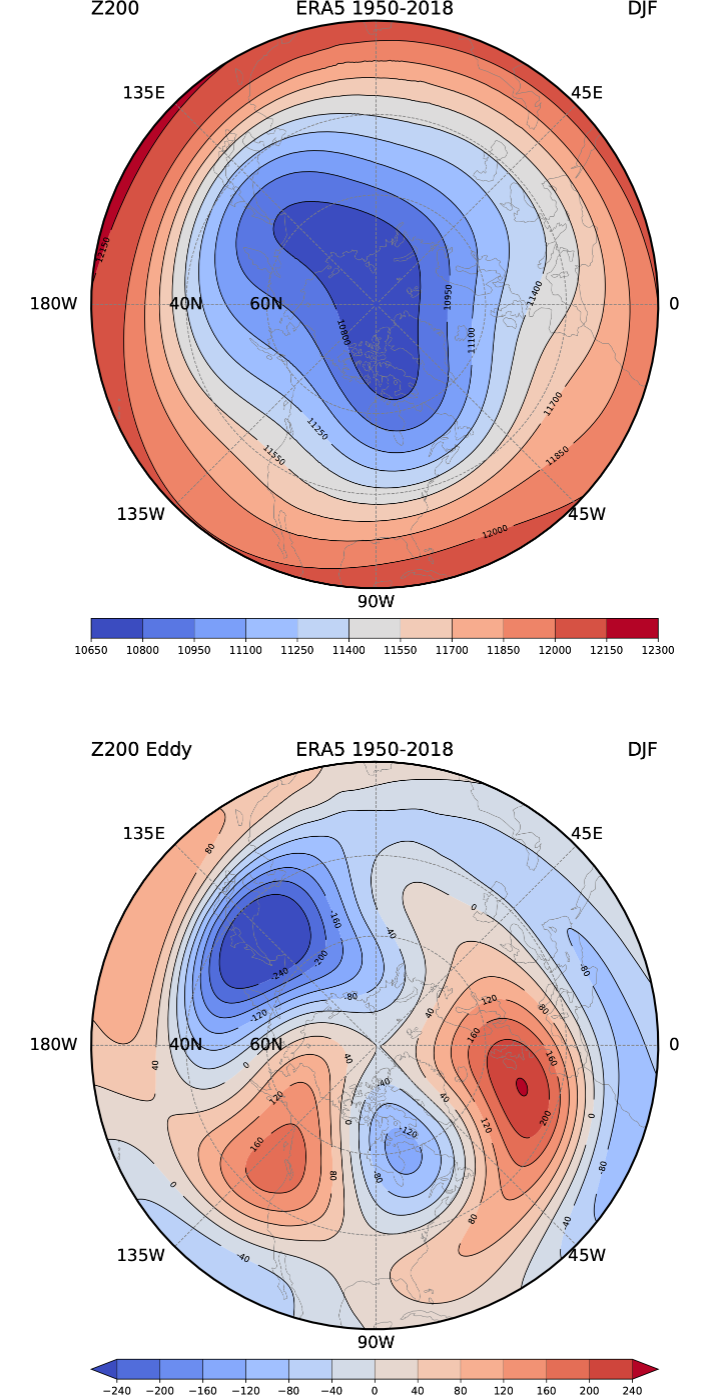
\includegraphics[width=0.5\linewidth]{uploads/Screenshot 2024-11-19 132440.png}
    \caption{Z200NH}
    \label{fig:enter-label}
\end{figure}


\subsubsection{The horizontal wind}\label{the-horizontal-wind}

The geopotential is a good approximation to the streamfunction in the
mid-latitudes where the geostrophic balance controls tightly the
dynamical balance, but it gives usa poor ideas of the wind circulation
in the low latitudes. In this case is better to look at the wind
directly. Fig. \texttt{fig:56} shows the zonal wind at 200mb for the
calendar Winter (DJF) and Summer (JJA). We can see clearly the westerly
jet streams in the winter of both hemispheres. The jets are concentrated
on the east coast of both large continental land masses.

The Asian jet is the most intense, reaching at its core a velocity in
excess of 70 m/s. In comparison, the North American jet is weaker and
smaller in longitudinal extent. The winter jet in the Southern
Hemisphere is also well formed, but at this level is not at the same
amplitude of the northern hemisphere jets. Summer westerly jets are also
present in both summer hemisphere, but much weaker.

The tropical region instead is characterised by easterly jets, most
prominent over the maritime continent and the equatorial South America.
In Summer the Easterly circulation over the Indian Ocean is very
intense. The longitudinal gradient of the wind implies areas of
divergent flow over South America and the Indonesian region.

The meridional wind in winter (DJF) (Fig. \texttt{fig:57}) shows the
alternating patterns of positive and negative (poleward and equatorward)
that are consistent with the eddy pattern of the geopotential. Large
deviations from the zonal mean occur over the Pacific-North American
sector and over Far East Asia. In the calendar Summer (JJA) the winds
are weaker and they reach a somewhat large amplitude only over the
southern hemisphere.

Close to the surface (Fig. \texttt{fig:55}) the zonal wind is in general
weaker over land, but stronger over the ocean, and it is clearly
westerly in the mid latitudes, whereas easterlies dominates the
subtropical zone, with the notable exception of the Indonesian Region,
also called the Maritime Continent, where is westerly. The combination
of Easterlies and Westerlies in the equatorial Pacific point to a near
surface convergence area somewhere in the Central Pacific Ocean.

In JJA the zonal wind shows the seasonal cycle and it gets strength in
the winter hemisphere, retaining the general features that we have seen
for the Winter. Note instead the strong westerlies in the Indian Ocean.
This is the first evidence of the seasonal monsoonal circulation in the
Indian subcontinent. The Easterlies south of the westerlies indicates a
possible circulation over the Indian Ocean basin.
\begin{figure}[h!]
    \centering
    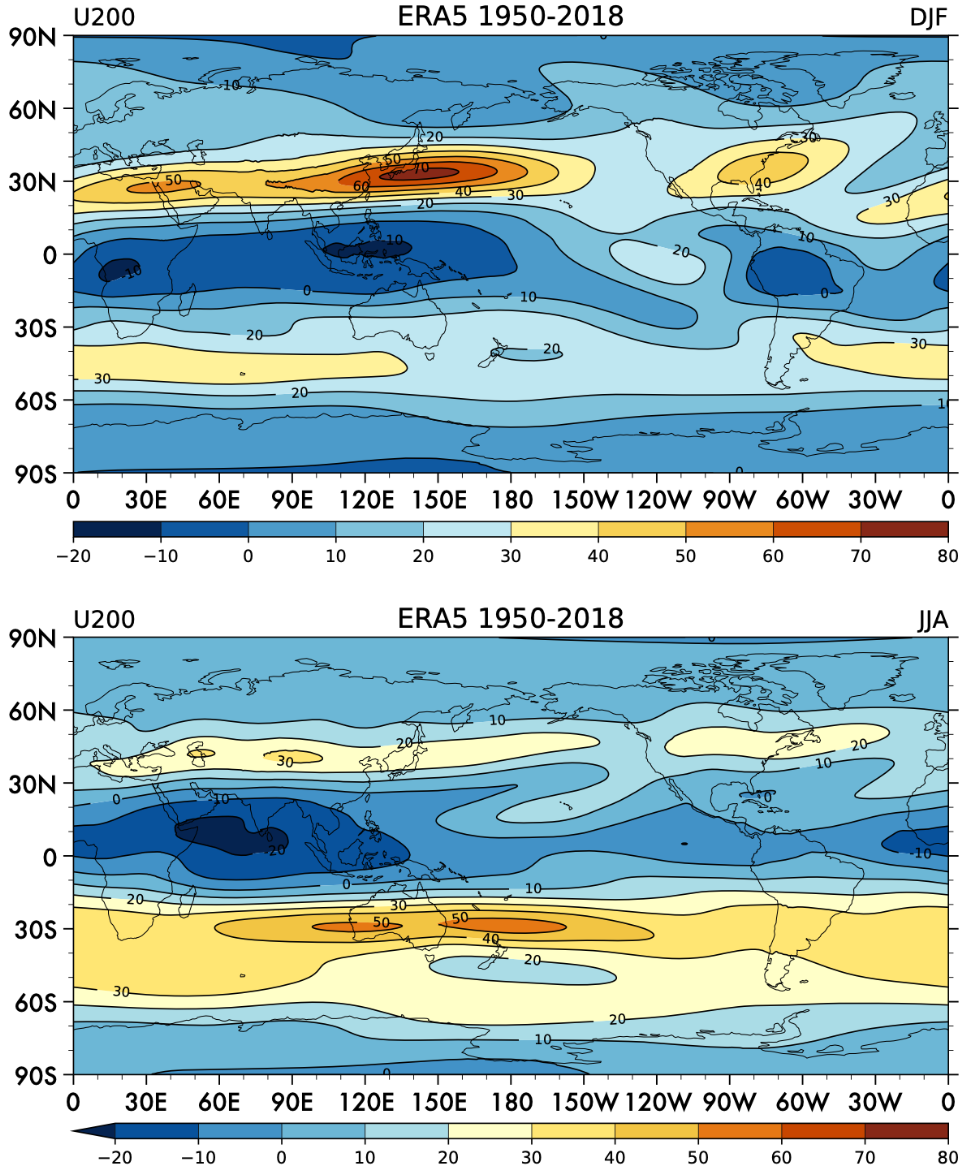
\includegraphics[width=0.5\linewidth]{uploads/Screenshot 2024-11-19 132557.png}
    \caption{U200}
    \label{fig:enter-label}
\end{figure}
\begin{figure}[h!]
    \centering
    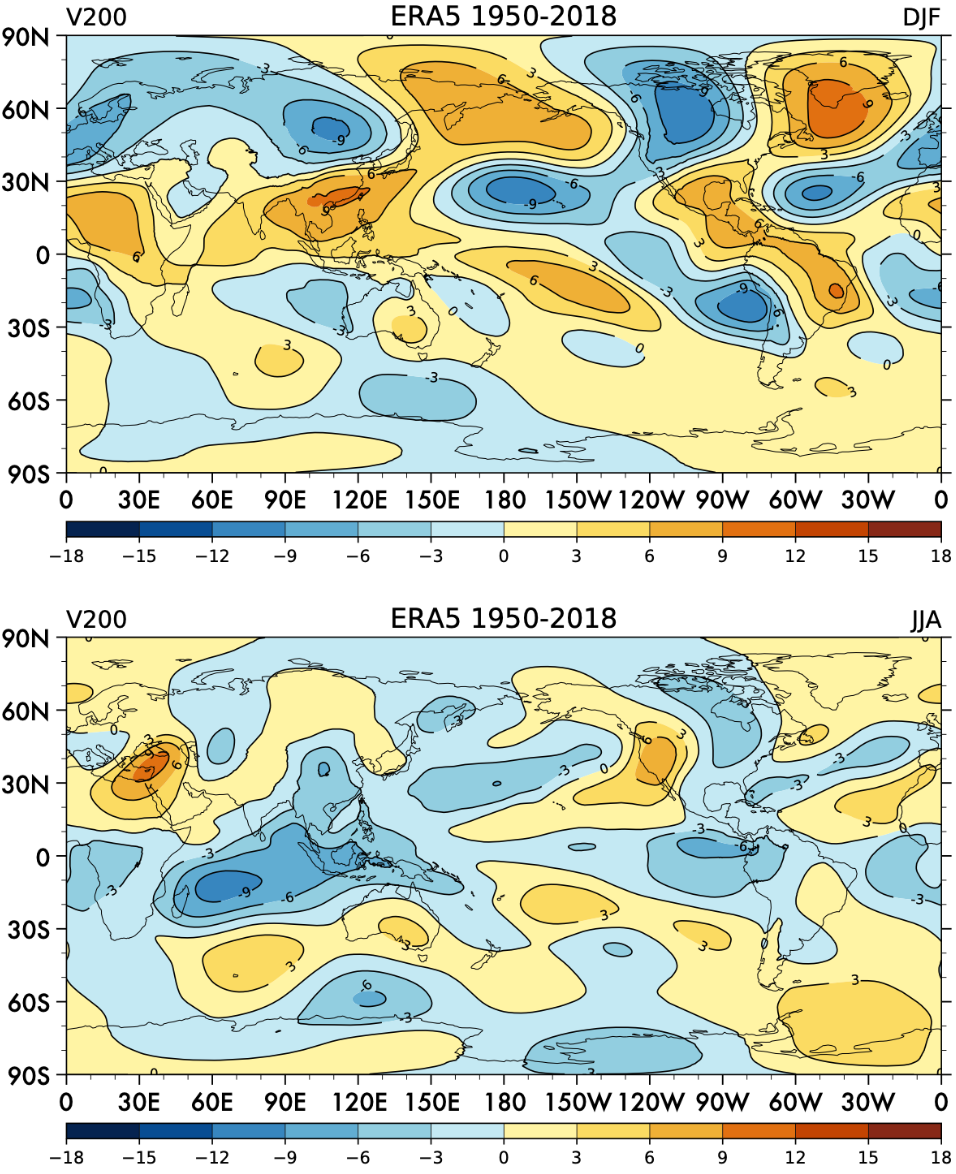
\includegraphics[width=0.5\linewidth]{uploads/Screenshot 2024-11-19 132652.png}
    \caption{V200}
    \label{fig:enter-label}
\end{figure}


The meridional wind near the surface (Fig. \texttt{fig:58}) shows
dramatic features. Neglecting the areas of high elevation (the Himalaya
plateau, Antarctica) where this pressure level is under ground and
therefore not particularly meaningful, we notice a systematic
equatorward flow over the east coast of continents. It is most intense
along South America, South Africa and the West African coast right North
of the Equator.

In Summer these along shore winds becomes more intense along the North
American and African coast. Interestingly, the flow is reverse along thr
Somali coast in the Indian Ocean. The meridional flow is reversed with
respect the Winter season. In the Summer it is easy to see that this
flow is closing the circle with the zonal flow in Fig. \texttt{fig:55}
creating a cyclonic circulation that is the distinctive tract of the
South Asian Monsoon.


\begin{figure}[h!]
    \centering
    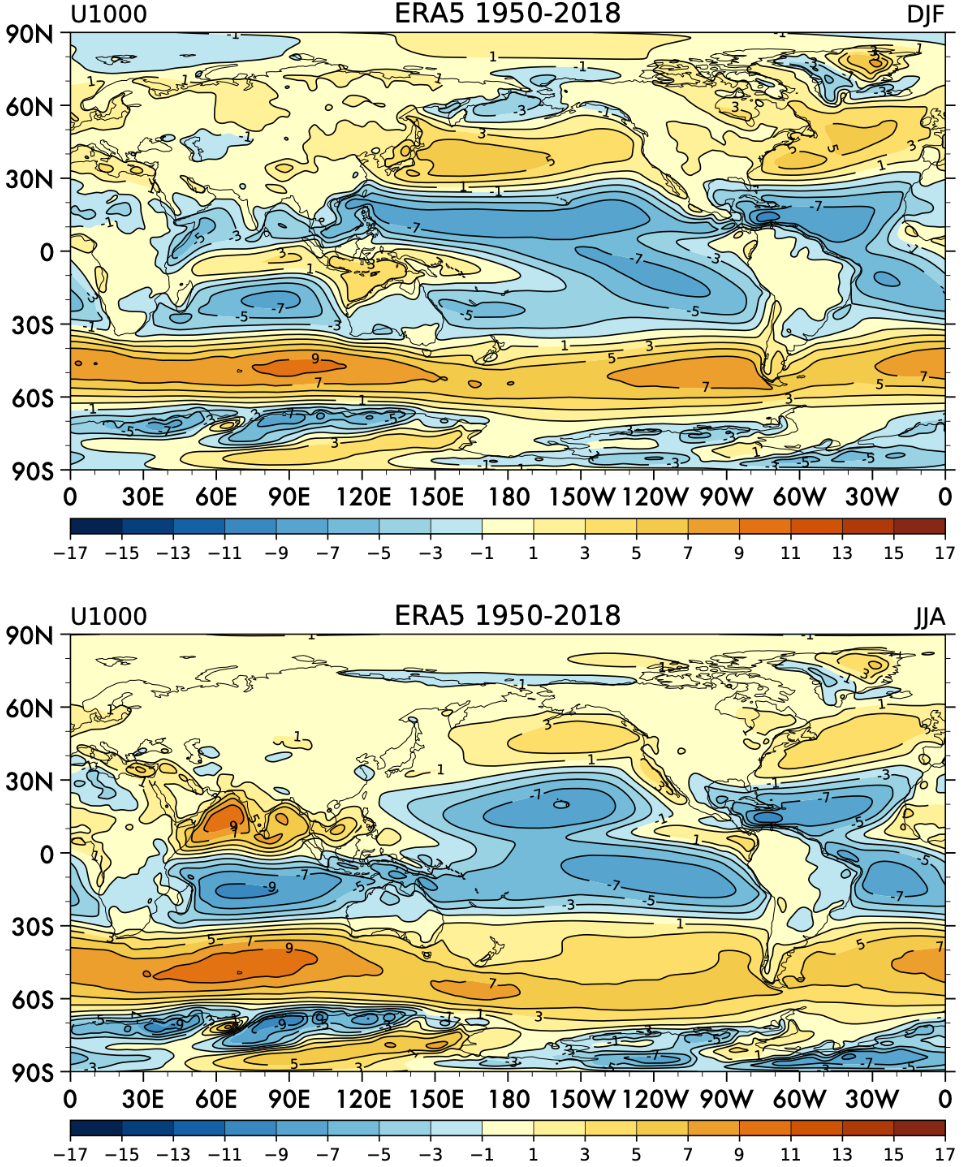
\includegraphics[width=0.5\linewidth]{uploads/Screenshot 2024-11-19 132853.png}
    \caption{U1000}
    \label{fig:enter-label}
\end{figure}
\begin{figure}[h!]
    \centering
    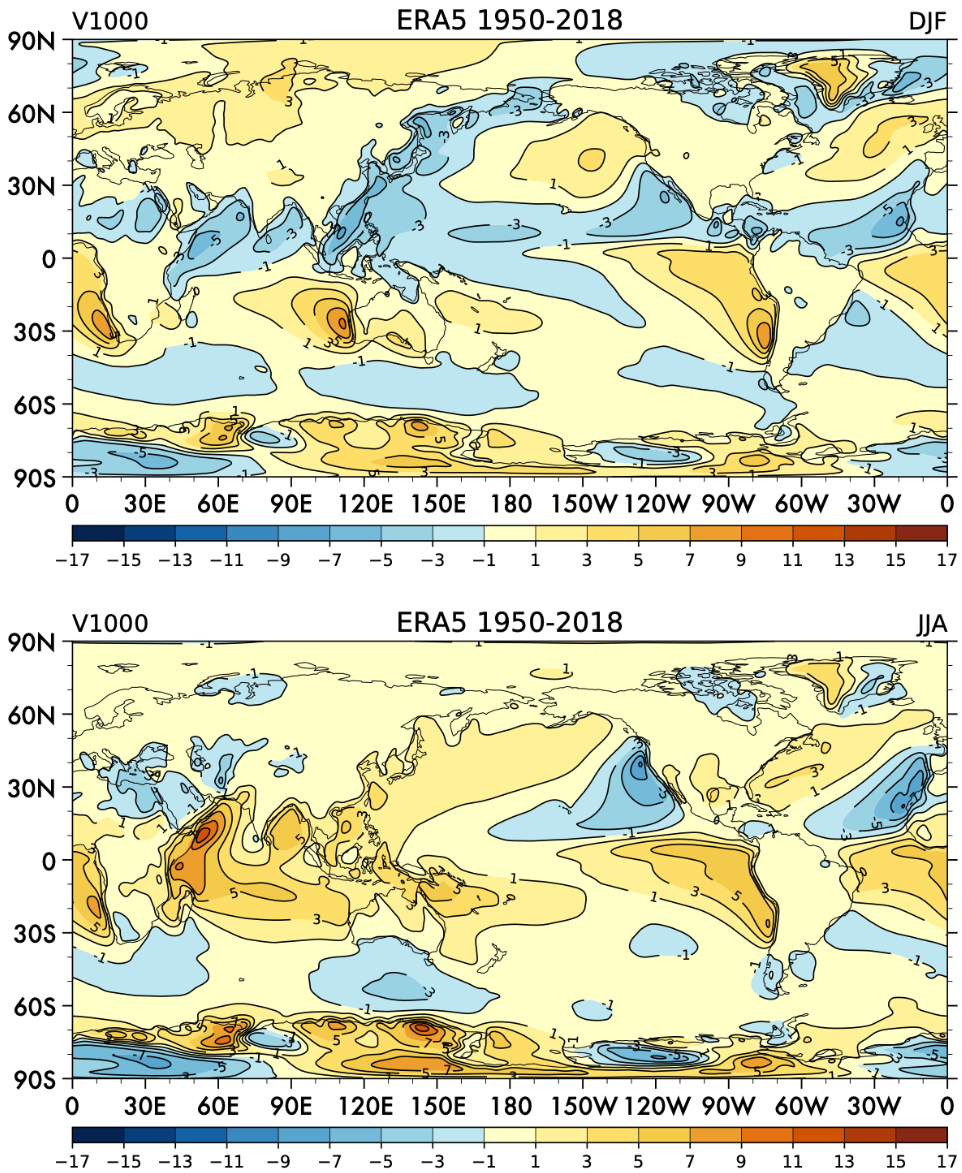
\includegraphics[width=0.5\linewidth]{uploads/Screenshot 2024-11-19 132750.png}
    \caption{V1000}
    \label{fig:enter-label}
\end{figure}

The \(1000mb\) circulation is very close to the ground and it represent
very well the forcing that the oceans feel from the atmosphere. As such
it is a crucial element of the interactions between atmosphere and
ocean. The real low- level circulation field for the atmosphere is
better represented by a level that is outside of the planetary boundary
layer over most of the planet surface. Such a level is traditionally
considered the \(850mb\) level.

Fig. \texttt{fig:580} shows the streamlines of the wind at 850mb level
in winter and Summer. The equatorial circulation is clearly visible in
the Pacific where the Trade winds cover the equatorial region, shifting
in latitude as they follow the seasonal cycle of the ITCZ. Large gyeres
circulation covers the ocean basin and the Asian Summer Monsoon
circulation in the Indian Ocean is clearly visible, curving from the
East Africa towards the Indian subcontinent and Indochina.

\begin{figure}[h!]
    \centering
    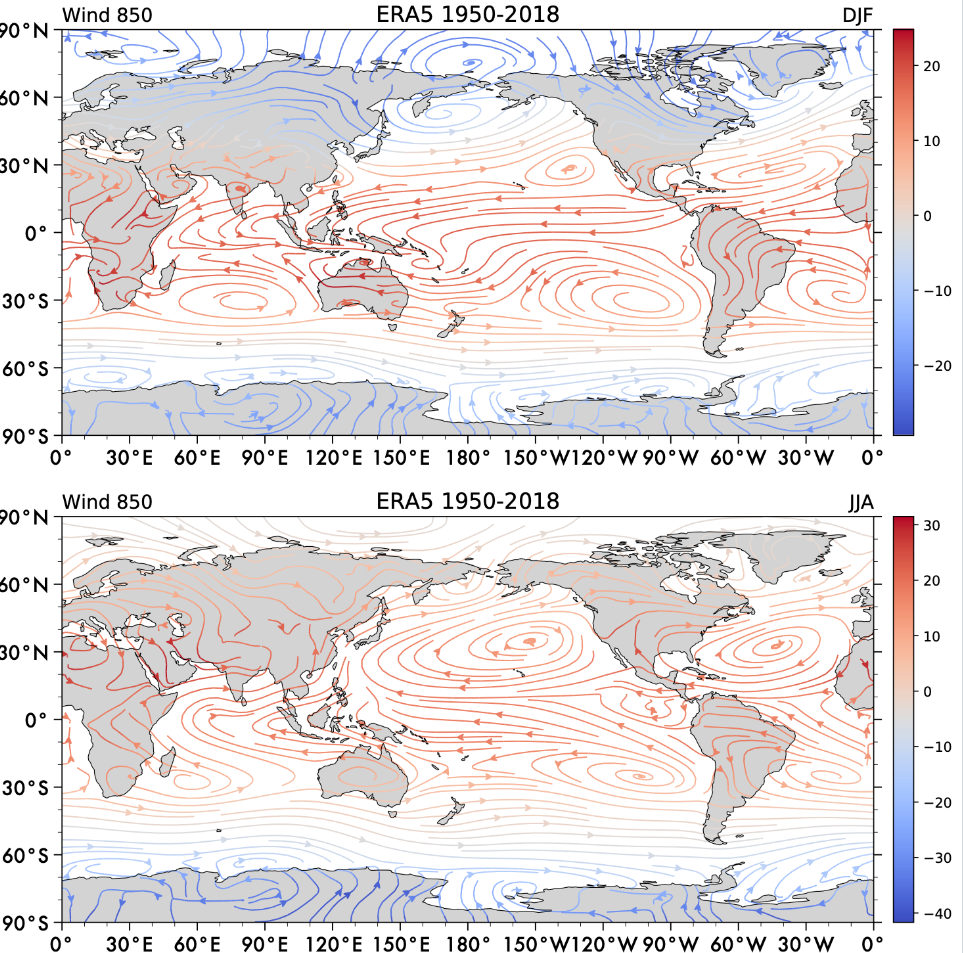
\includegraphics[width=0.5\linewidth]{uploads/Screenshot 2024-11-19 133008.png}
    \caption{Windo 850}
    \label{fig:enter-label}
\end{figure}


\subsubsection{Mean Sea Level Pressure}\label{mean-sea-level-pressure}

The distribution of Mean Sea Level pressure is another important
parameter to describe the general circulation of the atmosphere. This
field is obtained by calculating the pressure at the reference level for
the geopotential (zero level) that is conventionally considered the mean
sea level. It should better referred to as the reference geoid, but most
models still use a spherical Earth approximation, so the zero reference
can still be defined as a sphere.

The principal throwback is that this means that the areas of the Earth
where there are mountains the mean sea level is effectively underground
and therefore of limited usefulness. This especially evident for the
high mountain ranges, the Rockies and the Himalayas and for Antarctica.
Elsewhere, however, it gives a good description of the mass distribution
of the atmosphere. High values of mean sea level pressure correspond to
pile up of mass. The accumulation of mass is larger in the subtropics,
both in Winter and Summer, where a chain of high pressure centers is
present.

The picture is that there are three distinctively different region. The
Northern Hemisphere Midlatitudes, the intertropical region between the
Tropics and the midlatitudes of the Southern Hemisphere. The largest
seasonal contrast emerges in the northern hemisphere mid latitudes. Note
that in Winter high pressure tend to stay over the continent, whereas
low pressure centers develop over the ocean, in Summer it is the
opposite and high pressure stays over the continents.

The Intertropical zone is characterized by the presence of distinct high
pressure centers that oscillate with the season in latitude. The
Southern Hemisphere has a much more symmetric nature with a ring of low
pressure circling the Antarctic continent.

The seasonal cycle is visible in the shift of the ring of high pressure
at the rtropics in the north-south directions. Fig. \texttt{fig:59z}
shows the zonal and time mean for Summer and Winter of the meridional
distribution of sea level pressure. There is a general structure of high
sea level pressure in the tropics, with relative areas of low pressure
in the mid-latitudes and at the Equator. In the Southern hemisphere it
is ismuch more pronounced andf the gradients are much stronger. The
seasonal shift can be seen in the movement of tropical maxima.
\begin{figure}[h!]
    \centering
    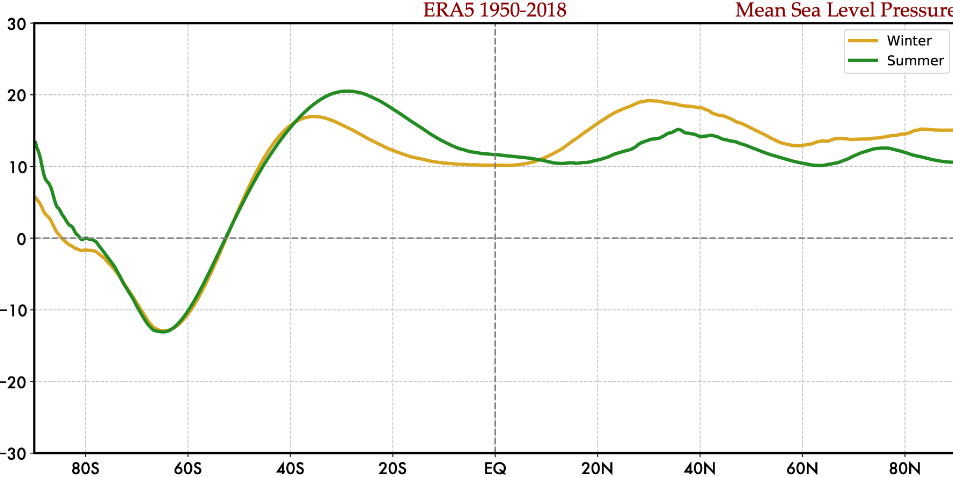
\includegraphics[width=0.5\linewidth]{uploads/Screenshot 2024-11-19 133117.png}
    \caption{MSLZONALDJF}
    \label{fig:enter-label}
\end{figure}


\subsubsection{The Sea Surface
Temperature}\label{the-sea-surface-temperature}

North-South gradients dominate the distribution of the Sea Surface
Temperature in both seasons (Fig. \texttt{fig:60}). Polar regions are
very cold and dominated by sea ice (not visible in this picture),
whereas the equatorial regions are generally very warm. However, there
are large deviation from the zonal symmetry close to the east cost of
continents. especially in the equatorial Pacific Ocean vast intrusions
of cold water are visible straight at the equator in the East Pacific,
where the water has the same temperature of the midlatitudes.

